\newpage
\section{Market Assessment}

Thus far, we have considered the technical capabilities and structure of our system. In this section, we show that it would be viable to bring our system to market. We explore trends and challenges in the shipping industry, and make predictions about its future growth. We then propose a market penetration strategy for OceanX, indicating how it might obtain trust and funding from other organisations. We conclude with a quantitative analysis of our proposed system, suggesting approximate operating costs and indicating how much up-front capital would be required to roll out our system in the countries we are targeting. 

\subsection{Industry Analysis}

The shipping industry consists of a number of freight companies, each providing transportation services to global exporters and importers. A typical interaction between a shipping company and goods producers is as follows. Goods importers will place an order with an exporting company, and exporters will then pay for storage and transfer of goods onto a ship, as well as any insurance required for the goods. The exporter will choose a shipping company based on the quoted freight rate, which indicates how much will be charged for the transportation of the goods. However, other considerations such as the quality of the insurance and transit time are important factors. 

The process of globalisation has caused rapid growth in international and intercontinental trade. With 90\% of all such trade conducted by sea \cite{IMOfacts}, the shipping industry has played, and will continue to play, a vital role in satisfying global demand. Figure \ref{fig:cargo_trends} shows the historical demand for cargo, along with the projected figures into 2030 and beyond. In almost all cases, an increase in the volume of cargo is expected. In particular, containerised shipping is expected to almost double in quantity in the next ~15 years.

\begin{figure}[h!]
	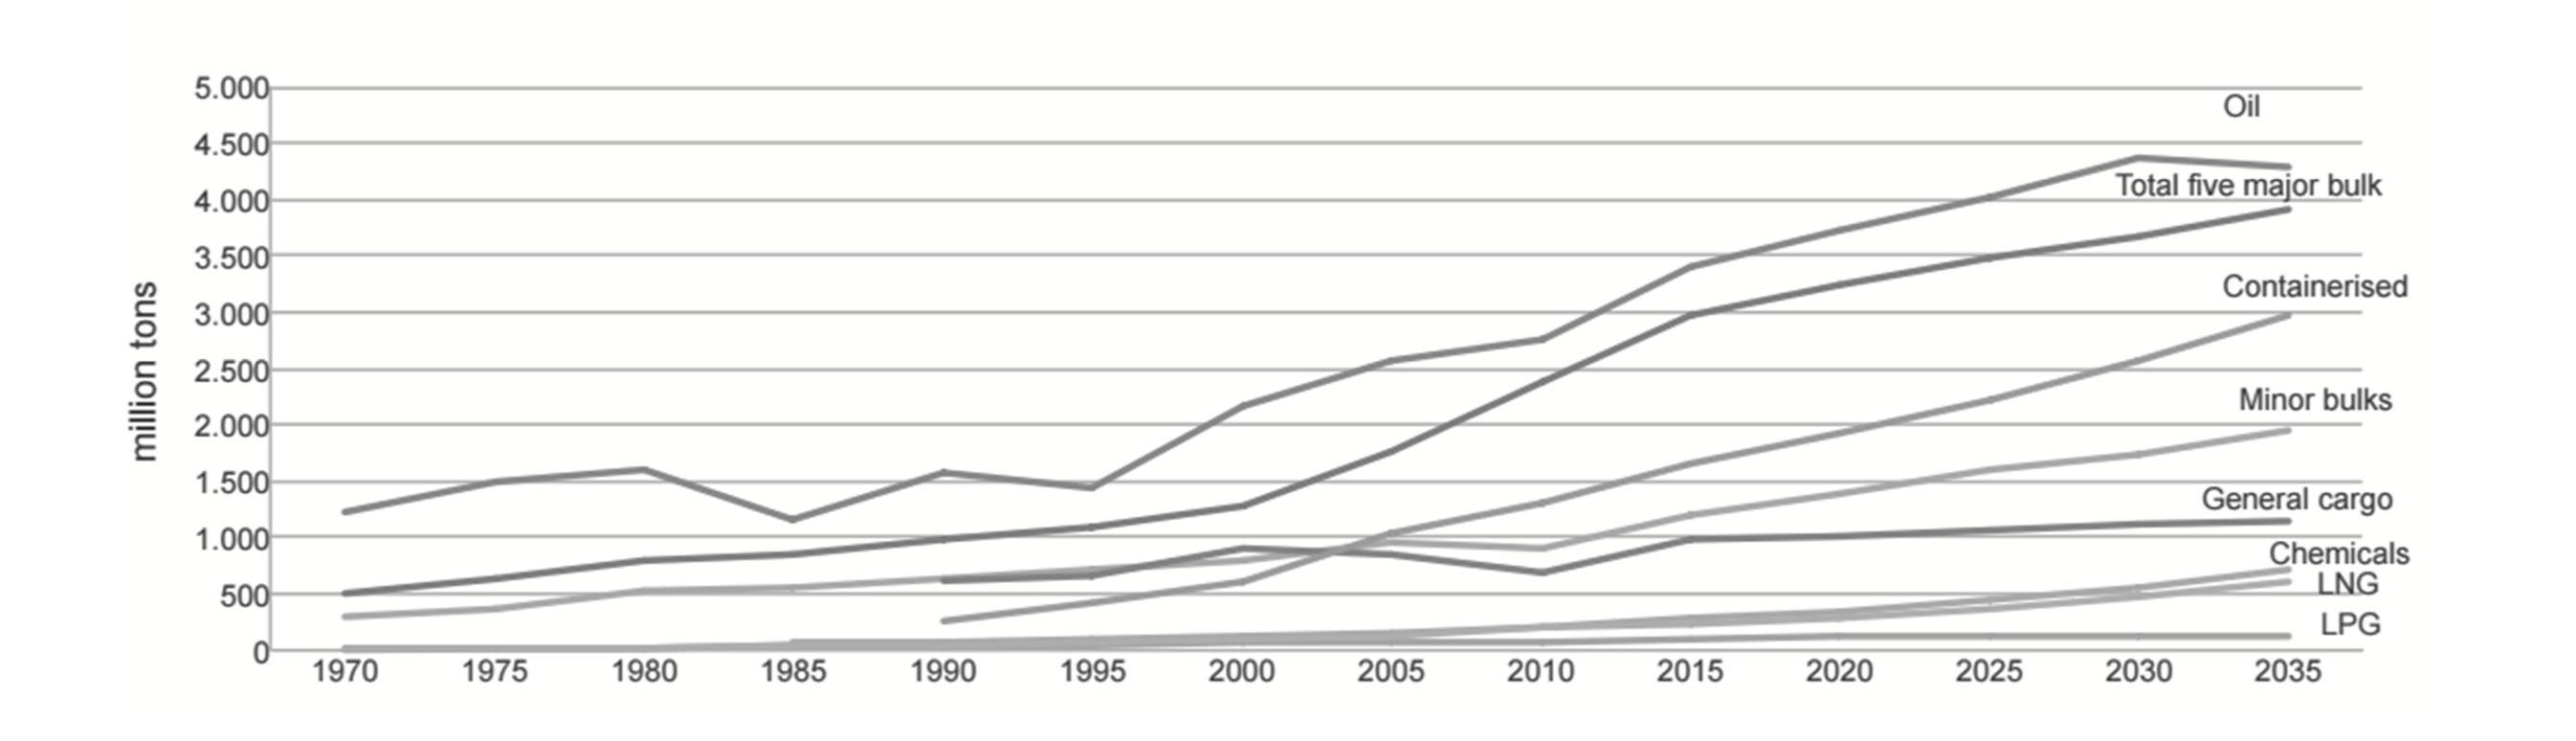
\includegraphics[width=\textwidth]{images/trade_trends}
	\caption{The trends in amount of cargo distributed globally, measured in millions of tons \cite{BluePlanet}.}
	\label{fig:cargo_trends}
\end{figure}

Despite this clear growth, the industry is arguably more sensitive to world events than most. For instance, Hanjin, a large Korean shipping company, was forced into administration in 2016 due to heavy drops in freight rates \cite{globalCrisis}. As well as danger from economic recession, the industry is somewhat unique in threats from piracy, often involving crew kidnapping with heavy human and economic costs. In addition, the industry must comply with environmental regulation from political bodies, which seek a 40\% reduction in carbon emissions by 2050 \cite{EUReduceEmission}.

Alphaliner provides data on the split of market share of top shipping companies with respect to the total cargo capacity, measured in Twenty-foot Equivalent Units \cite{LargestShipping}. The biggest players in the shipping industry are APM-Maersk, Mediterranean Shipping, CMA CGM Group, and COSCO Shipping. Together, they constitute  around 50\% of the market. Much of the success of the `big 4' is attributed to their ability to manage costs through efficient organisation and conservative development of ship capabilities \cite{MaerskMoney}, with the opportunity cost of additional business.

A key trend in shipping industry is a drive for more efficient ships with greater capacities in order to combat falling freight rates \cite{sizematters}. These larger ships are not without their own problems, since they require significant changes to port side infrastructure  in order to be sustainable \cite{ftarticle}. As an alternative to this heavy investment, ultra-deep water ports have been deployed, which have the advantage of accommodating the depth requirements of larger vessels. The UK government has considered the commisioning of an offshore deepwater port for the purpose of decommissioning the North Sea oil operation \cite{ConservativeManifesto}.

Another important trend in the short to medium term is the emergence of ``big data”. Firstly, the recently deployed Automated Identification System of satellites offer greater monitoring of ship positions and weather conditions. This allows for the informed route planning \cite{5trends}. Secondly, big data will be used to improve the visibility of market and pricing trends, stabilizing freight rates, and avoiding cases such as Hanjin in 2016. 

Finally, further adoption of autonomous systems is expected in the medium to long term. Rolls-Royce is beginning this process with a global research project ultimately aiming to deploy a fully autonomous system by the end of the decade \cite{autoboats}. The main advantage of the autonomous approach is the cost saving in reduction in required crew size. However, fully autonomous systems still require occasional human maintenance. Autonomous systems address the problem of piracy, by removing the opportunity to hold human lives hostage \cite{SOS}.


\subsection{Market Penetration Strategy}

We envision that the system will be  deployed initially at a single location. In other words, we propose one offshore smart port servicing multiple land ports with a fleet of autonomous shuttle ships. To determine the path to realising this goal, we have identified the key players in bringing the OceanX system into the shipping industry. 

The company (OceanX) shall work with companies who wish to move goods (exporters) by offering freight and cargo insurance services in competition with existing freight companies. To the exporter and importer, there will be no additional steps required in order to use the OceanX system. On successful bid for exported goods, our fleet of autonomous shuttle ships will transfer the cargo from the coastal port to the offshore port. Next, in order to transfer the goods onward to their destination, we will employ services of the existing shipping providers  using a portion of the fee levied on the exporter. The large intercontinental cargo ships will dock at our offshore ports instead of a coastal port. For importing, we shall have a similar relationship with the freight companies. Large freight ships will deliver cargo bound for multiple coastal destinations to the offshore port, then the fleet of autonomous ships will be deployed to forward cargo to the specific coastal destination.

The primary motivation for the competition to use our system, instead of docking at coastal ports, is the ability for larger ships to be serviced. This enables higher utilisation of ship resources, since cargo from many coastal ports can be coalesced at a single offshore port. This allows our competition to continue the trend of building larger ships at higher cost effectiveness, while allowing OceanX to avoid heavy investment in the newest and largest freight ships. The fleet of autonomous ships will initially consist of repurposed freight vessels.  Ultimately, we hope to build our own ships with autonomous control in mind, allowing maximal use of space and energy. However, significant initial cost savings can be made through adaptation of existing resources. 

We will seek co-investment for the construction of the offshore port. As mentioned, the UK government has already expressed interest in building such a port. Additional funds can be raised by partnering with existing freight companies in exchange for priority/preferred usage rates. Additional sources of revenue come from the use of the offshore port by non-OceanX vessels. For instance, the air solution developed by Team A involves making long flights over water, and our offshore ports may be used to charge these aircraft for a fee. In addition, fuelling and docking services will be charged to freight ships using the system.

Crucially, we shall build trust with the exporter, freight companies, and wider public. To this end, the system will be rolled out incrementally, with a strong focus on reliable and secure operation. Initially, the system may function as a single offshore port and a small repurposed fleet. To gain the trust of exporters we shall offer a generous insurance policy on the transfer of goods, with our liability kept low by the fact that goods are transferred at the offshore port. In addition, we will promote the autonomous aspect of the system in enhancing user privacy, lowering the risk of piracy for the exporter by removing the possibility of human hostage taking. To gain the trust of freight companies we may simply point to the cost efficiency gains from allowing the trend of larger ships to continue.

Development of the initial port and fleet should continue until the company builds significant trust and market share, as measured by the number of containers moved in our serviced region. At this point, we will seek further  governmental/competitor investment to franchise or co-develop additional OceanX systems around the world.

At this stage, the main goals of the project would be achieved. However, once the network of OceanX systems is established, there is scope to expand the capabilities of the company. Firstly, purpose built autonomous shuttle ships would be developed for coastal to offshore delivery. In addition, OceanX may explore the use of its own intercontinental autonomous freight ships to “cut out the middleman”, triggering competition with existing freight companies which are already deeply invested in the OceanX system.

We believe the key threat to our deployment plan is that historically, the shipping industry has been reluctant to embrace new technology -- instead opting to stick with tried and tested economics. This is evident just by observing the slow pace at which Maersk and other big companies upgrade their fleets to larger, more cost-effective vessels. As mentioned previously, in order to address this threat, we would seek to initially partner with government programmes focusing on the development of offshore ports. This reluctance to innovate, however, can also be viewed as a key opportunity for OceanX. In particular, since existing companies can dock at our offshore ports without modifying their ships, they can retain their current model without being held back by a lack of shore-side investment.


\subsection{Quantitative Market Analysis}

As outlined in the industry analysis, revenues in the shipping industry have fluctuated significantly in recent years. The Great Recession caused a substantial reduction in the rate of growth of the volume of cargo shipped, which in turn has hurt the profits of major shipping lines through a “prolonged slump in the shipping market” \cite{ShippingSlump}. Despite this downturn, however, the 4 largest shipping lines still collectively generate \$75bn in annual revenue \cite{TroubledWaters}. One contributing factor to this decline is that in order to maximise efficiency, lines have invested in larger ships, with modern vessels having 30\% greater capacity (20,000 TEUs) than those from before the Great Recession (15,000 TEUs) \cite{ftarticle}. This means that despite efficiency savings through an increase in vessel capacities, the availability of cargo space has often exceeded demand. This has lead to crashes in freight prices.

With the volume of cargo doubling by 2030 \cite{BluePlanet}, it is reasonable to assume the revenue for the industry will increase by a similar amount, in addition to price increases caused by inflation. Furthermore, we assume the response by the shipping industry will be to continue investment in larger ships.

As the number of high-capacity ships increases, substantial investment on port side resources will be needed to meet demand. The OceanX system reduces pressure on existing coastal ports, and enables investment from these ports to be redirected into a single local offshore port. Assuming the costs of our offshore port solution will be approximately equal to that of a typical oil rig, we expect that each offshore port will require a capital investment of around £500m \cite{MaerskRigs}. However, we aim to recycle materials from decommissioned oil rigs as the world becomes less reliant on fossil fuels. With regards to the investment required to  develop our fleet of autonomous shuttle ships, either new vessels can be commissioned, or used ships can be retrofitted. As such, it is estimated the average cost of a ship will be in the region of £1-2.5m \cite{forsale}, excluding any specialist autonomous control hardware.

As well as the initial development costs, there will be daily costs to maintain and run the fleet of ships and the offshore port. Based on operating costs for similarly-sized ships today, we estimate initial daily operating costs totalling £30k per ship \cite{DailyOperatingCostsShips} and £500k for the offshore port \cite{DailyOperatingCostsOilRig}. These values are based on existing ships and semisubmersibles, and therefore are pessimistic cost projections. Two major cost reductions will come from the reduced number of personnel, and the use of renewable energy.

We anticipate that the main source of revenue for the OceanX system shall be the fees we collect from exporters, in addition to fees from import contracts for moving goods from our offshore ports back to coastal ports. Freight rates vary based on destination, we would expect to charge between £500 and £3000 per container \cite{ContainerRates}. We would like to generate additional revenue through dockside services, such as refueling and charging. 

In summary, the initial aim of the OceanX deployment plan is to secure trust and financial investment from the key stakeholders such as government, coastal port operators, and shipping companies. To begin with, we will begin to draw market share from businesses wishing to export products with a competitive insurance and freight rate package. While we expect substantial up-front costs in development and procurement, we believe that the long-term cost savings of our approach will lead to rapid growth and eventual world wide adoption of the OceanX system.
